\section{Aufbau des Clients}

Aus den oben genannten Anforderungen kann eine grobe Architektur abgeleitet werden.
Zur Realisierung des Observerpatterns wird die sigc++ library benutzt die mit Gtkmm kommt.
Es wird empfohlen die Einführung bis einschließlich Kapitel 2 zu lesen:
\begin{itemize}
\item \url{http://developer.gnome.org/libsigc++-tutorial/stable/ch01.html}
\end{itemize}
Die ersten Einsätze werden auch noch tiefer erklärt.

\newpage
\subsection{Hauptklassen}
\begin{figure}[htb!]
	\centering
        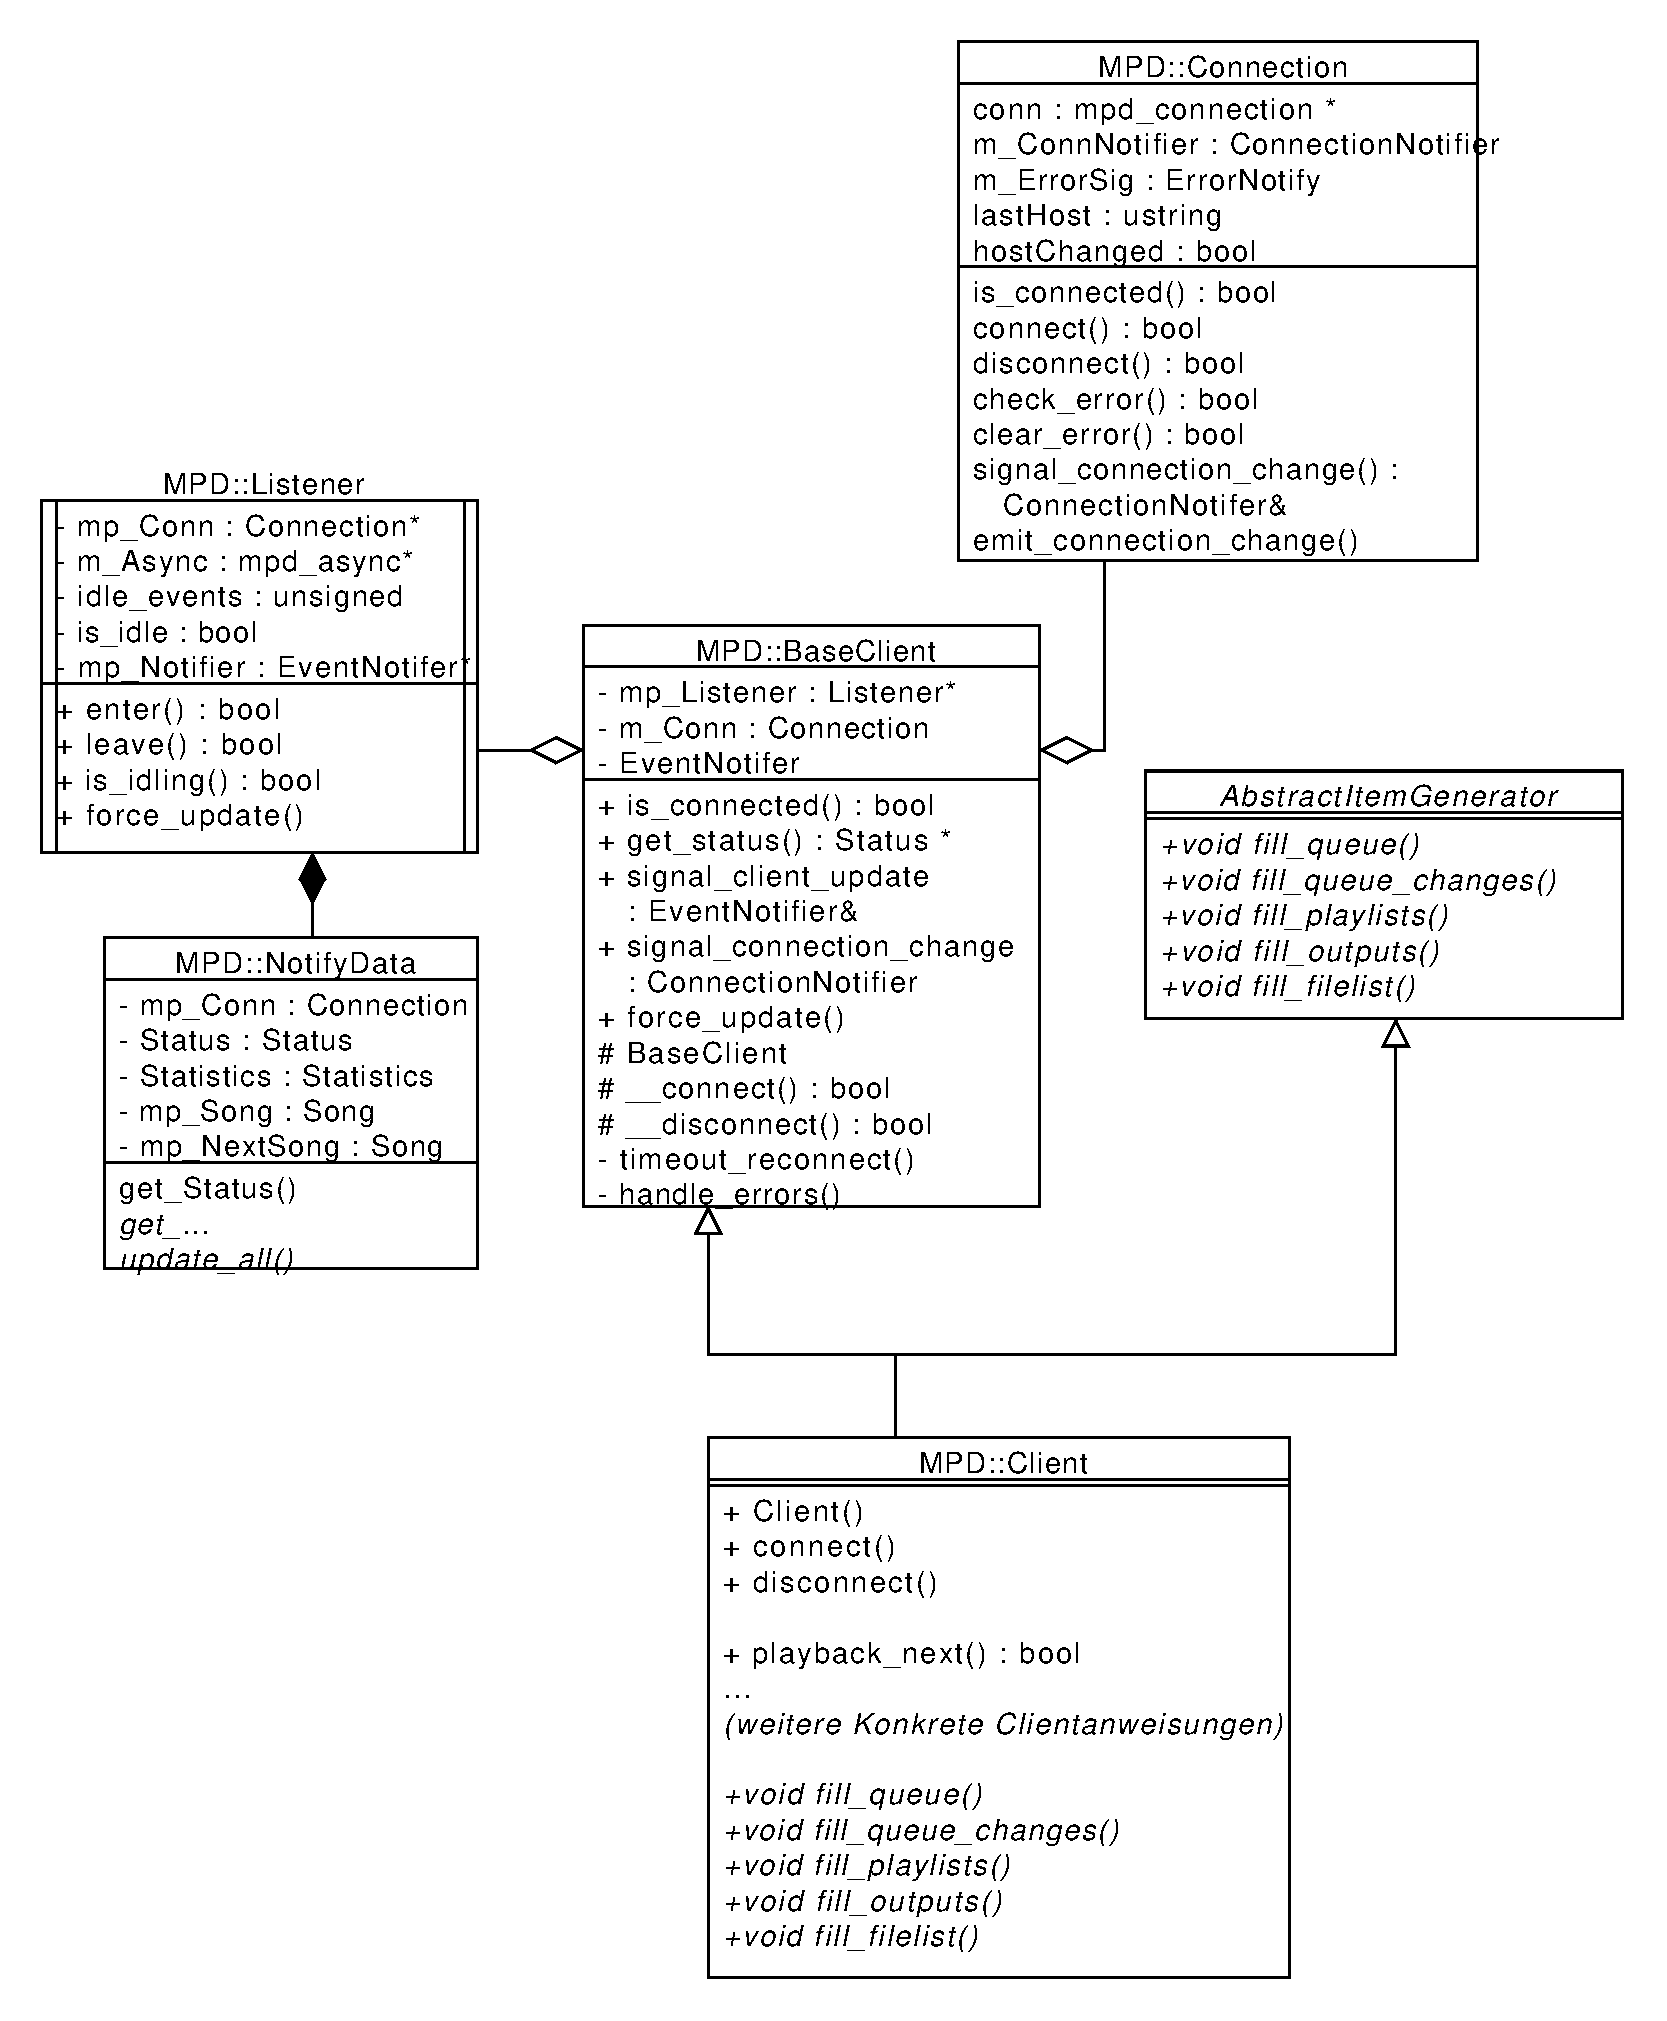
\includegraphics[scale=0.5]{ClientCollab.pdf}
	\caption{Übersichtsklassendiagramm zur Clientstruktur}
	\label{class_client_all}
\end{figure}

\newpage
\subsubsection{Listener}
\begin{figure}[htb!]
	\centering
        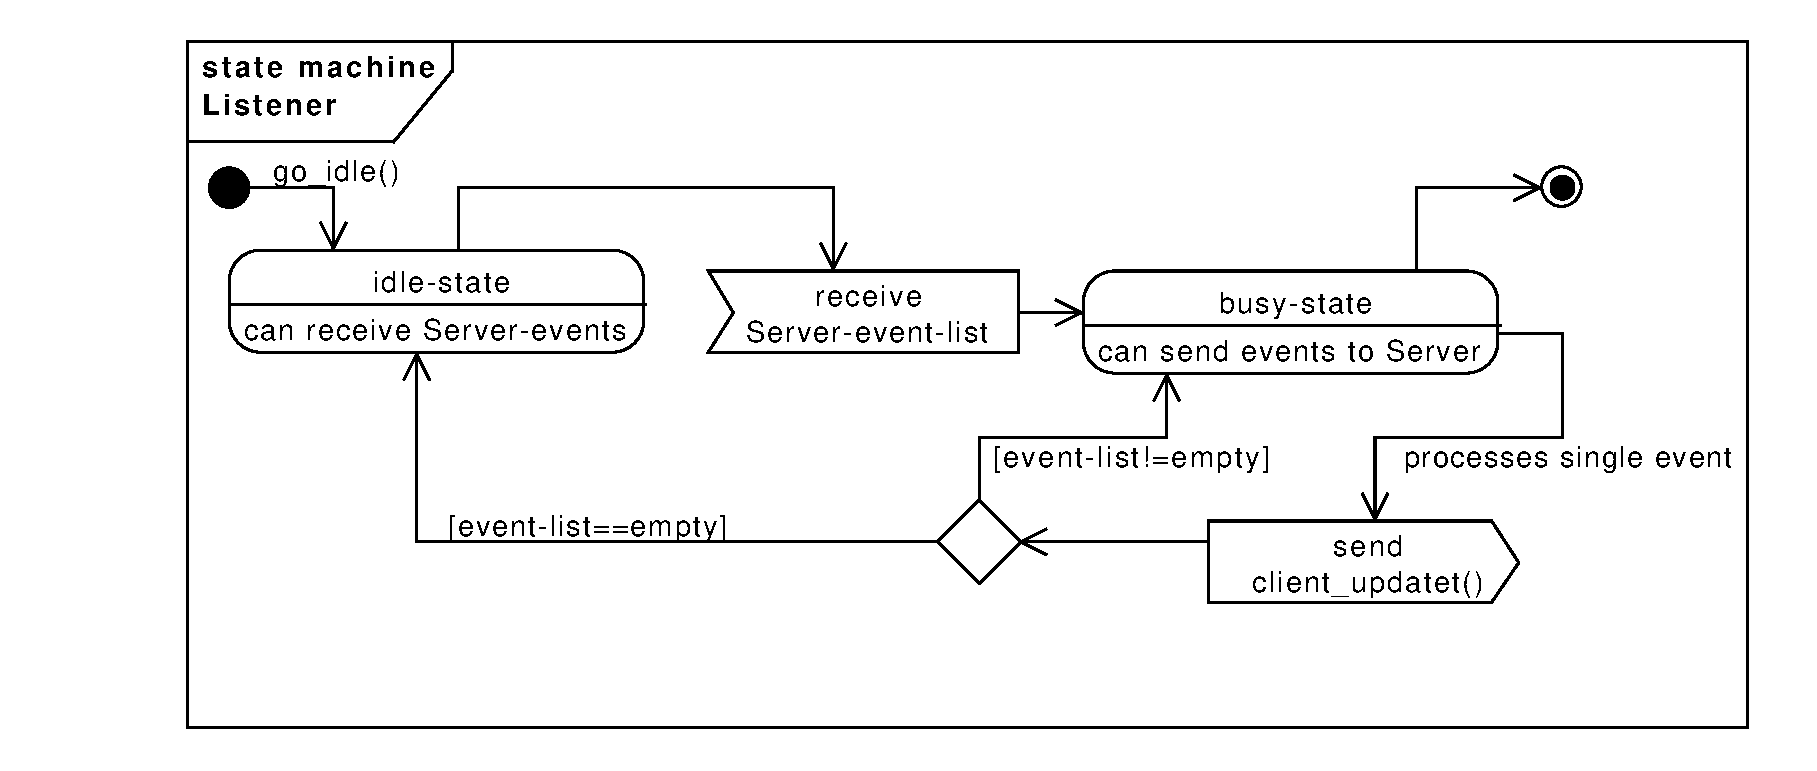
\includegraphics[width=\textwidth]{st_ListenerIdleBusy.pdf}
	\caption{Zustandsdiagramm Listener ,,idle/busy''}
	\label{st_listener}
\end{figure}

Der Listener verwaltet alles was mit dem Betreten und Verlassen des ,,Idlemodes'' und den damit verbundenen Events
zu tun hat. Er setzt den eingangs beschriebenen ,,Watchdog'' auf die asynchrone Verbindung an,
und ,,parst'' die entsprechenden Antworten des Servers von Hand (siehe \ref{st_listener}). 
\\
\\
Es folgt eine Liste aller möglichen Events die von libmpdclient definiert werden.
Die Aktionen die passieren müssen, damit diese eintreten, stehen in Klammern.
\begin{itemize}
    \item \small MPD\_IDLE\_DATABASE \it(Datenbank hat sich geändert)\rm
    \item \small MPD\_IDLE\_STORED\_PLAYLIST \it(Änderung an den Playlisten)\rm
    \item \small MPD\_IDLE\_QUEUE \it(Änderung an der Queue: Clear, Add, Remove)\rm
    \item \small MPD\_IDLE\_PLAYER \it(Pause,Stop,Play,Next,Stop,Previous,Seek)\rm
    \item \small MPD\_IDLE\_MIXER \it(Änderung an der Lautstärke)\rm
    \item \small MPD\_IDLE\_OUTPUT \it(An/Ausschalten eines Outputs)\rm
    \item \small MPD\_IDLE\_OPTIONS \it(Random,Repeat,Single,Consume)\rm
    \item \small MPD\_IDLE\_UPDATE \it(Datenbankupdate/rescan wurde gestartet)\rm
\end{itemize}
\normalsize
Bei der Instanzierung des Listeners soll das \textit{sigc::signal} welches das Clientupdate darstellt übergeben werden.
Zudem benötigt der Listener eine Referenz auf MPD::Connection um an die darunter liegende asynchrone Verbindung zu kommen.  
\begin{verbatim}
  Listener(EventNotifier& Notifier, Connection& sync_conn);
\end{verbatim}

Eine weitere Aufgabe des Listeners ist es, das Model MPD::NotifyData aktuell zu halten. Siehe dazu auch MPD::NotifyData.
Bemerkt der Listener Events so ruft er emit() auf dem übergebenen \textit{sigc::signal} auf,
und übergibt als Parameter das aufgetretene Event, sowie eine Instanz von MPD::NotifyData.
\footnote{Als spätere Optimierung könnte das aufgetretene Event übergeben werden um selektiv Daten ,,upzudaten''; Sprich bei einer Lautstärkeänderung muss kein neues Statistikobjekt geholt werden.}
\\
Es folgt eine Liste von Funktionen die der Listener mindestens haben soll.
\\
enter() tritt in den ,,Idlemode'' ein. Es ist ab diesem Punkt nicht mehr erlaubt Kommandos zu senden.
leave() ist das genaue Gegenteil von enter() und verlässt den ,,Idlemode'' sodass Kommandos gesendet werden können.  
is\_idling() sollte selbsterklärend sein.
\begin{verbatim}
       bool enter(void);
       void leave(void);
       bool is_idling(void);
\end{verbatim}

Es soll zudem eine force\_update() Funktion geben die ,,künstlich'' alle Events auslöst.
Dies ist nützlich bei der Initialisierung, bzw. bei ,,Reconnectvorgängen'', wenn die GUI gezwungen werden
soll sich zu updaten.
\begin{verbatim}
       void force_update(void);
\end{verbatim}

\subsubsection{Connection}
\begin{figure}[htb!]
	\centering
        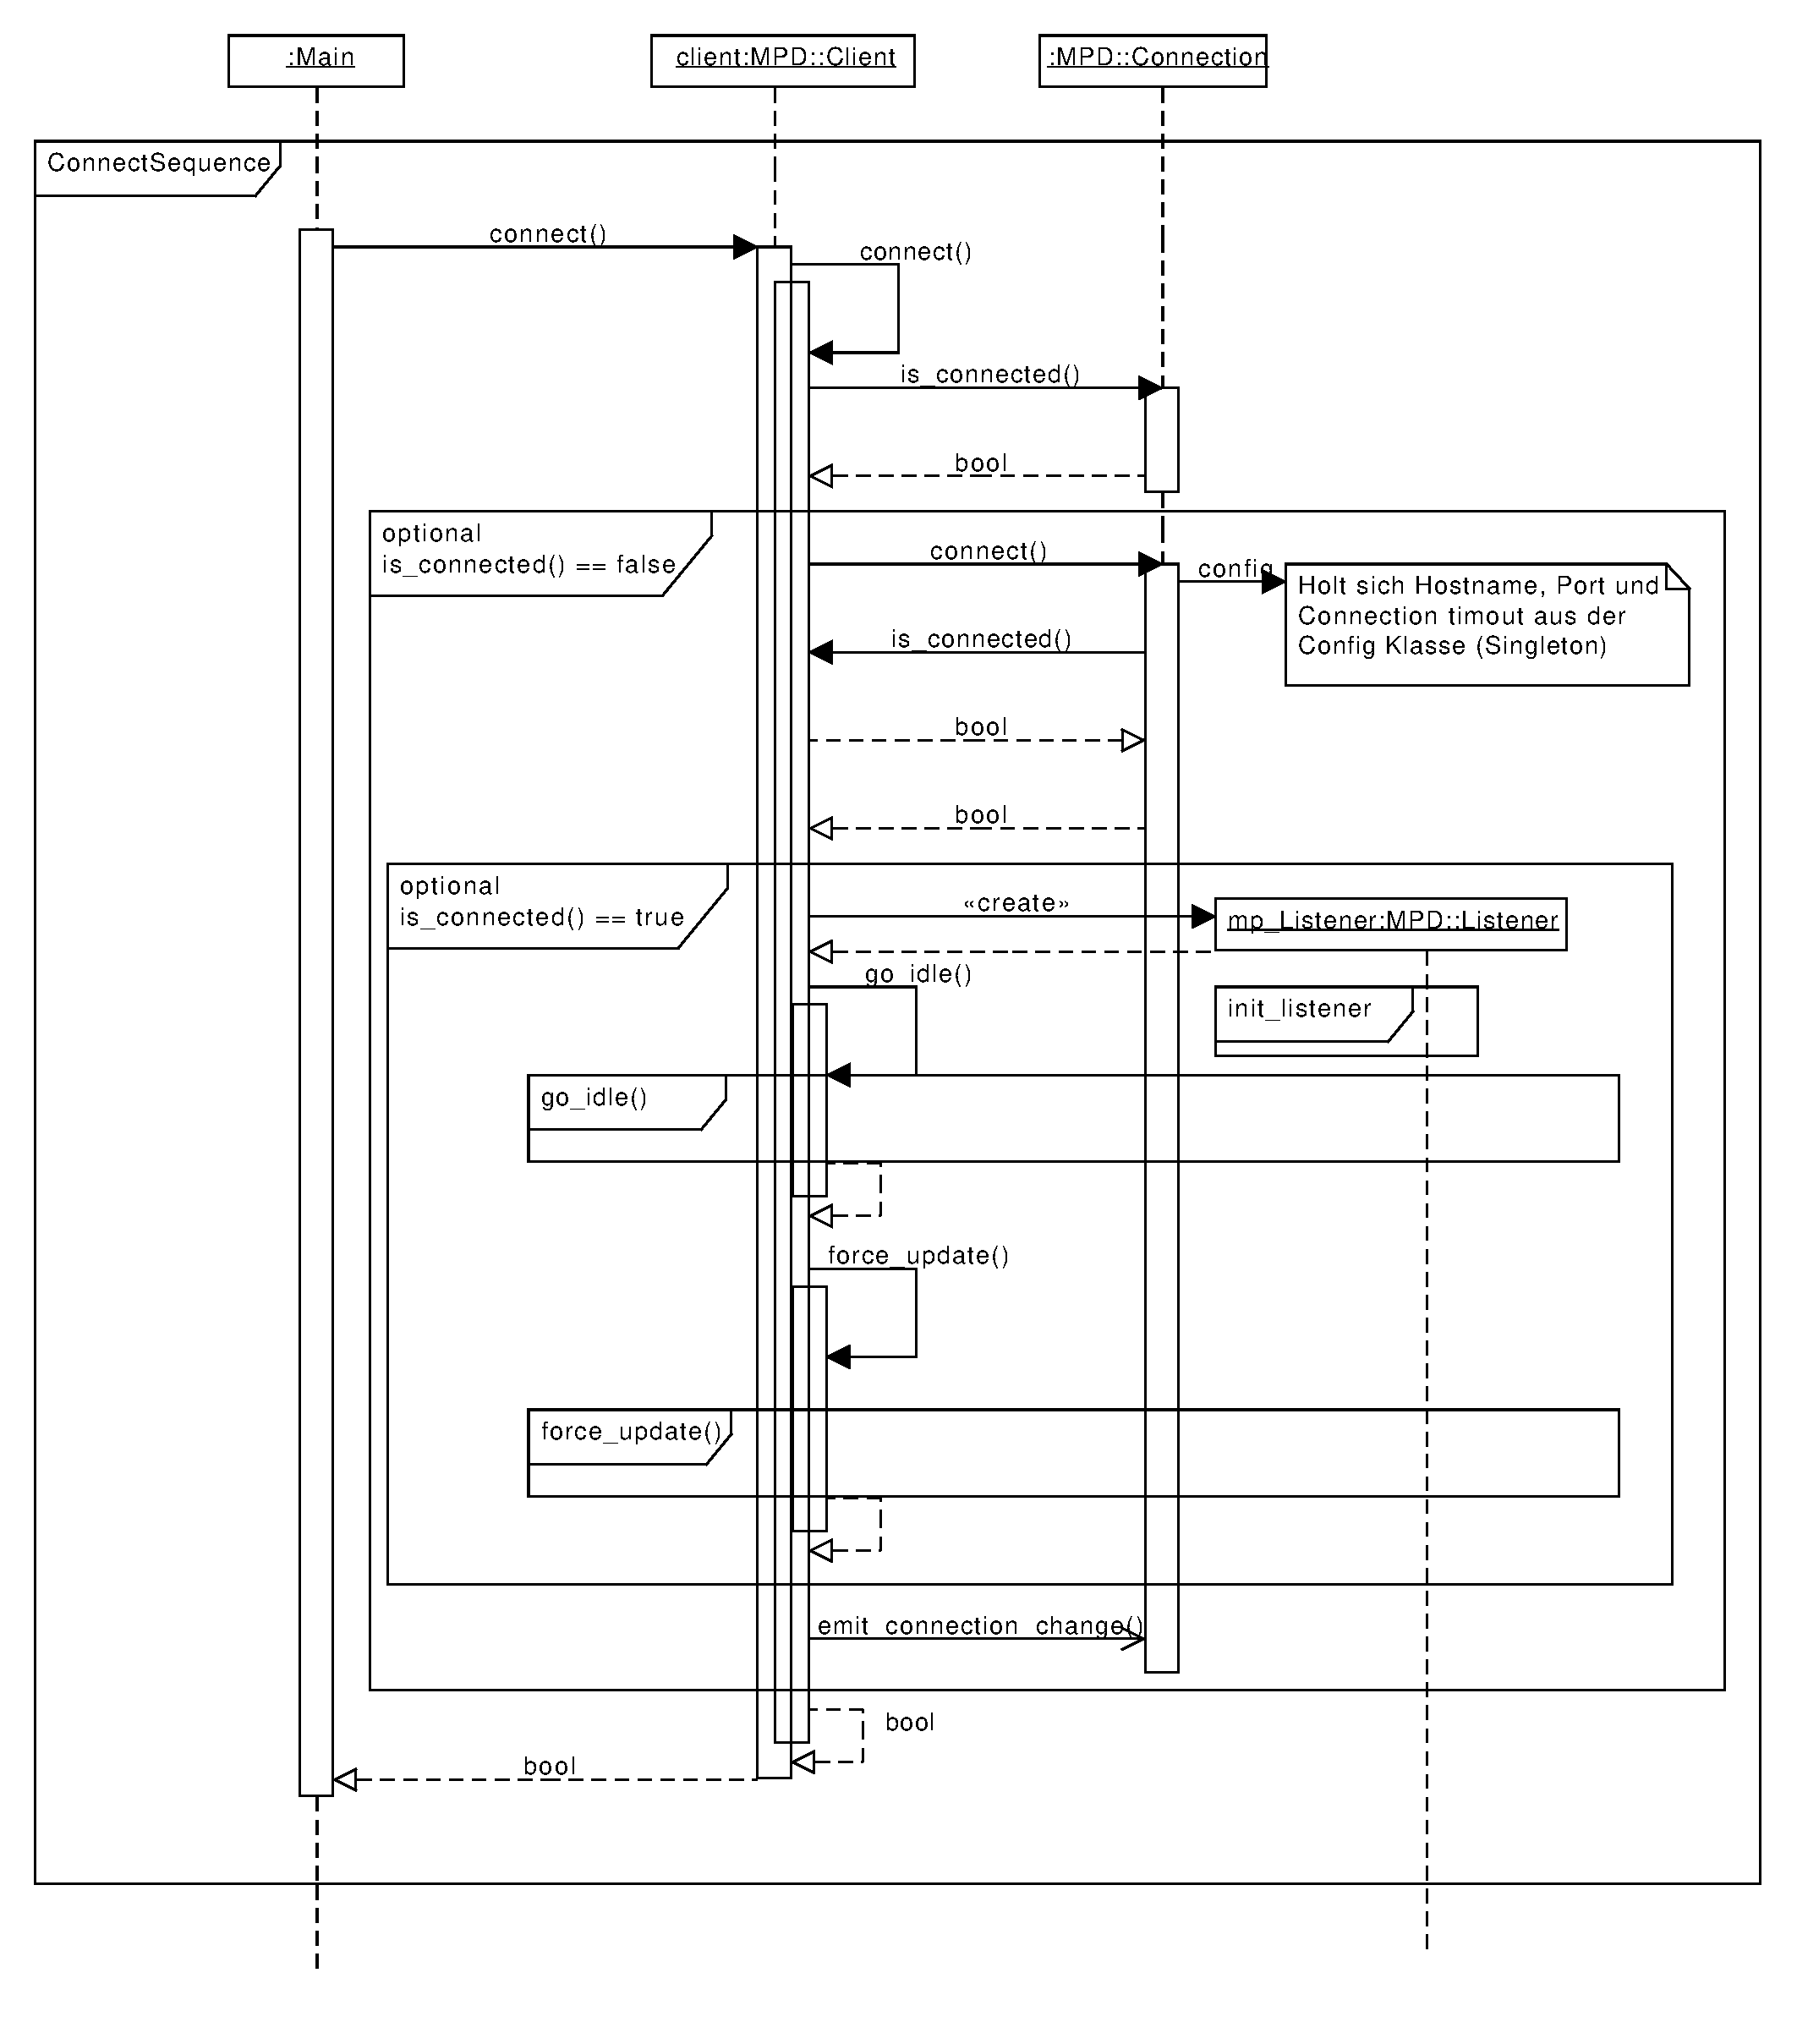
\includegraphics[scale=0.5]{ConnectSequence.pdf}
	\caption{Sequenzdiagramm zum Verbindungsaufbau}
	\label{seq_client_connect}
\end{figure}
Diese Klasse stellt eine Art Wrapper um die \textit{mpd\_connection}
\footnote{http://www.musicpd.org/doc/libmpdclient/connection\_8h.html} Struktur von libmpdclient da.
Sie bietet die ,,eigentlichen'' connect() und disconnect() Methoden die letzlich \textit{mpd\_connection\_new()} bzw. \textit{mpd\_connectio\_free()} aufrufen. Siehe \ref{seq_client_connect} für den detaillierten Verbindungsablauf. Die benötigten Verbindungsdaten (Host, Port, Timeout in Sekunden) holt sich MPD::Connection aus der Config.
\\
Sie hält zudem den letzten Host als Membervariable um feststellen zu können ob sich dieser zwischen 
zwei Verbindungsvorgängen geändert hat. Desweiteren bietet sie eine Schnittstelle um andere Klassen über Fehler in der Verbindung informieren zu lassen (signal\_error()), bzw. um sie zu ,,reparieren'' (clear\_error()).
\\
Es folgt eine Liste von Funktionen die mindestens vorhanden sein sollten.
Ein boolean-Rückgabewert von true zeigt stets Erfolg an.
\\
connect() soll die eigentliche Verbindung herstellen, disconnect() löscht die Verbindung wieder.
get\_connection() liefert einen Pointer auf die darunter liegende C-Struktur.
Alle 3 Funktionen prüfen zudem intern bereits auf Fehler. 
\begin{verbatim}
    bool is_connected(void);
    bool connect(void);
    bool disconnect(void);
\end{verbatim}

Zur Implementierung konkreter Kommandos wird die darunterliegende C-Struktur benötigt.
\textbf{Siehe auch:} AbstractClientExtension
\begin{verbatim}
    mpd_connection * get_connection(void);
\end{verbatim}

Die Connectionklasse soll zudem Schnittstellen bieten um sich für Fehler- und Verbindungsänderungen
zu registrieren. 
Auf den Rückgabewert der folgenden Funktionen kann sigc::signal::connect() aufgerufen werden,
um einen Funktionspointer zu registrieren der aufgerufen wird sobald ein Fehler eintritt,
bzw. sich die Verbindung ändert. Die Schnittstellen sollen wie folgt aussehen:
\begin{verbatim}
  typedef sigc::signal<void, bool,mpd_error> ErrorNotify;
  typedef sigc::signal<void,bool,bool> ConnectionNotifier;
    
  ErrorNotify& signal_error(void);
  ConnectionNotifier& signal_connection_change(void)
\end{verbatim}

Die Prototypen entsprechen stets den Templateargumenten in den typedefs:
\begin{verbatim}
  void error_handler(bool is_fatal, mpd_error err_code);
  void conn_change_handler(bool server_changed, bool is_connected); 
\end{verbatim} 

Siehe MPD::BaseClient weiter unten für ein Beispiel wie eine Callbackfunktion registriert wird.
\\
libmpdclient verbietet es weitere Kommandos an den Server zu senden wenn vorher ein Fehler passiert ist.
Fehler müssen zuerst mit \emph{mpd\_connection\_clear\_error()} ,,bereinigt'' werden, 
dies tut check\_error(). Die Funktion wird normal nicht selbst aufgerufen, da sie von allen anderen Funktionen der Klasse
implizit aufgerufen wird. Ist ein Fehler passiert so werden alle Klienten die sich zuvor
mit signal\_error() registriert haben benachrichtigt. 
\begin{verbatim}
  bool check_error(void);
\end{verbatim}

\begin{figure}[htb!]
	\centering
        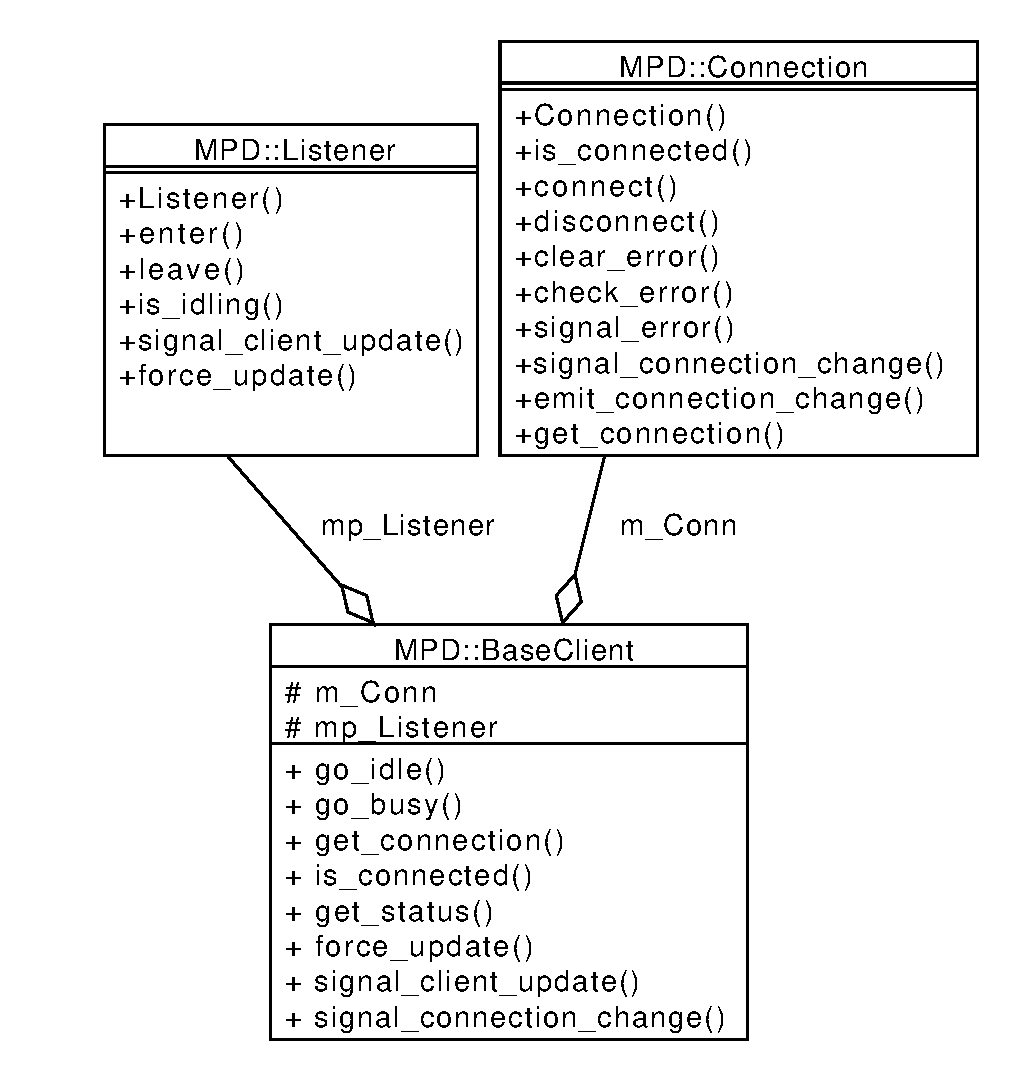
\includegraphics[scale=0.55]{BaseClientCollab.pdf}
	\caption{Klassendiagramm zu BaseClient}
	\label{collab_base_client}
\end{figure}

\newpage
\subsubsection{BaseClient}

\begin{figure}[htb!]
	\centering
        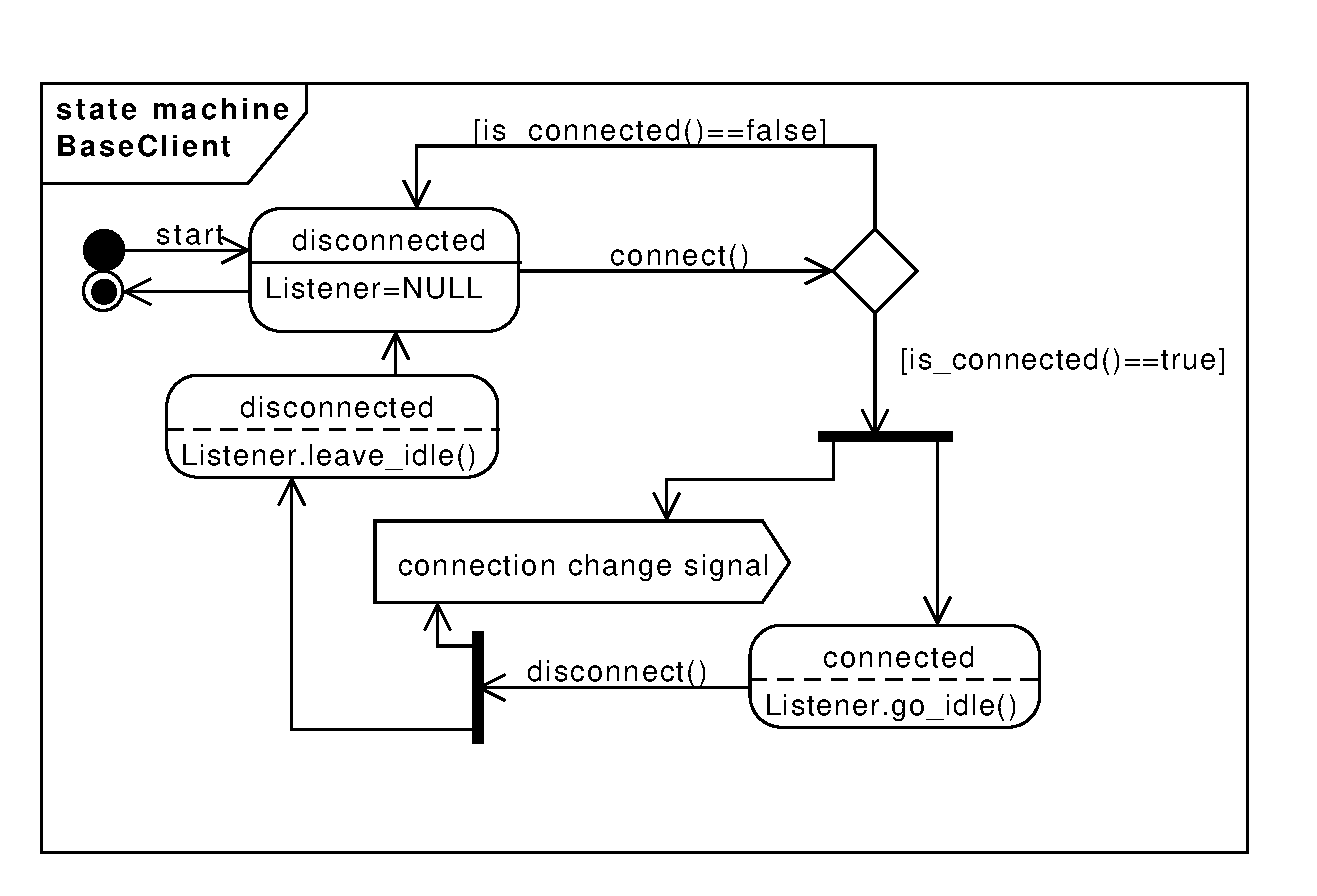
\includegraphics[width=\textwidth]{st_BaseClientConnection.pdf}
	\caption{Zustandsdiagramm BaseClient Connection}
	\label{st_base_client}
\end{figure}

Diese Klasse bildet die Basis zum eigentlichen Client. Sie kann nicht direkt instanziert werden, da
der Konstruktor protected sein soll.
Sie verwaltet administrative Tätigkeiten wie den eigentlichen Verbindungsaufbau an sich (siehe \ref{seq_client_connect} und \ref{st_base_client}). 
Desweiteren bietet die Klasse einfache Methoden zum Eintreten (go\_idle()) und Verlassen (go\_busy()) des ,,Idlemodes'' an.
Geht die Verbindung verloren, ohne dass \emph{\_\_disconnect()} explizit aufgerufen wurde, so wird versucht sich periodisch zu reconnecten.
Das Intervall in dem diese Versuche geschehen sollen, soll von ,,settings.connection.reconnectinterval'' gelesen werden.
\\
\\
\textbf{Siehe auch:} AbstractClientExtension
\\
MPD::BaseClient soll mindestens folgende public Methoden bieten:
\\
Gibt eine Referenz auf das zugrunde liegende MPD::Connection Objekt zurück. 
Siehe AbstractClientExtension für eine detailliertere Erklärung.
\\
\begin{verbatim}
  Connection& get_connection(void);
\end{verbatim}

Gibt \textit{true} zurück wenn eine Verbindung besteht.
\begin{verbatim}
   bool is_connected(void);
\end{verbatim}

Die get\_status() Funktion soll den letzten aktuellen MPD::Status zurückliefern,
oder \emph{NULL} falls nicht verbunden. Es soll garantiert sein, dass stets ein MPD::Status vorliegt,
wenn is\_connected() wahr ergibt.
\begin{verbatim}        
   Status * get_status(void);
\end{verbatim}

Die folgenden Methoden bieten eine Möglichkeit sich für Clientevents (signal\_client\_update()),
 bzw. für Verbindungsänderungen (signal\_connection\_change()) zu registrieren. 
\begin{verbatim}
  typedef sigc::signal<void,mpd_idle,MPD::NotifyData&> EventNotifier;
  EventNotifier& signal_client_update(void);
        
  typedef sigc::signal<void,bool,bool> ConnectionNotifier;
  ConnectionNotifier& signal_connection_change(void);
\end{verbatim}

Registrieren kann man sich über die sigc::signal::connect() Methode:
\begin{verbatim}
 // Callback Funktion wird bei jedem eingetretenen Event aufgerufen
 void on_client_update(enum mpd_idle event, MPD::NotifyData& data)
 {
    // Tue etwas bei einem 'player' event
    if(event == MPD_IDLE_PLAYER)
    {
        // Gib den Namen des aktuellen Songs aus
        cerr << data.get_song().get_path() << endl;
    }
 }

 // Registrieren der Callbackfunktion
 // - Ableiten von AbstractClientUser macht dies automatisch
 m_Client.signal_client_update().connect(sigc::ptr_fun(on_client_update));
\end{verbatim}

Folgende 3 Funktionen funktionieren genau wie enter(), leave() und force\_update() des Listeners,
allerdings prüfen sie mit Connection::check\_error() vorher stets auf Fehler.
\begin{verbatim}
  void go_idle(void);
  void go_busy(void);
  void force_update(void);
\end{verbatim}

%
%
%
% Zustands oder Sequenzdiagram zum Ausfürehn eines beliebigen Kommandos
% Sprich: go_busy( ) -> send command -> go_idle( )
%
\subsubsection{Client}
Der Client erbt von BaseClient und implementiert konkrete Kommandos wie ,,play'',,,random'' etc.
Er bietet zudem Schnittstellen zur Befüllung der Datenbank, der Queue und des Playlistmanagers indem 
er die abstrakte Klasse \emph{AbstractClientExtension} ausimplementiert.
Er bietet die Methoden connect() und disconnect() die letzendlich von Anwendern der Clientklasse zum Verbinden und Trennen genutzt werden. 
Ist in der config ,,settings.connection.autoconnect'' gesetzt, so connected er sich automatisch.
\\
\\
connect() und disconnect() stellen die öffentliche Schnittstelle zum Verbinden dar.
Sie rufen intern lediglich \_\_connect() bzw. \_\_disconnect() von MPD::BaseClient auf.
\begin{verbatim}
    void connect(void);
    void disconnect(void);
\end{verbatim}

Der Client soll eine Reihe von Kommandos bereitstellen um das Playback zu kontrollieren.
Die ersten 5 der folgenden Funktionen sollten relativ klar sein. 
Zu playback\_pause() sei angemerkt, dass es bei Wiedergabe anhält und bei keiner Wiedergabe wie playback\_play() funktioniert.
playback\_seek() springt in den Song mit der ID song\_id an die Stelle abs\_time in Sekunden.
Die ID des momentan spielenden Songs kann durch get\_status() gefunden werden.
Alle Funktionen, mit Ausnahme von playback\_crossfade), lösen ein ,,player'' Event aus. 
playback\_crossfade löst hingegen ein ,,options'' Event aus.
\begin{verbatim}
    void playback_next(void);
    void playback_prev(void);
    void playback_stop(void);
    void playback_play(void);
    void playback_crossfade(unsigned seconds);    
    void playback_pause(void);
    void playback_seek(unsigned song_id, unsigned abs_time);
    void playback_song_at_id(unsigned song_id);
\end{verbatim}

Die folgenden Funktionen dienen dazu jeweils die \it random, consume, repeat\rm und \textit{single}-modi umzuschalten.
Alle lösen ein ,,options'' Event aus.
\begin{verbatim}
    void toggle_random(void);
    void toggle_consume(void);
    void toggle_repeat(void);
    void toggle_single(void);
\end{verbatim}

Desweiteren sollten Methoden zum Bearbeiten der Queue vorhanden sein.
\begin{itemize}
    \item \textbf{queue\_add():} Fügt rekursiv den Pfad in der Datenbank hinzu. queue\_add(``/'') entspricht der ganzen Datenbank.
    \item \textbf{queue\_clear():} Leert die gesamte Queue.
    \item \textbf{queue\_delete():} Leert den Song ander Position 'pos'
    \item \textbf{queue\_save\_as\_playlist():} Speichert die aktuelle Queue als Playlist mit dem Namen 'name'
\end{itemize}
\begin{verbatim}
    void queue_add(const char * url);
    void queue_clear(void);
    void queue_delete(unsigned pos);
    void queue_save_as_playlist(const char * name);
\end{verbatim}

database\_update() sendet MPD Server Hinweis um DB zu aktualisieren.
database\_rescan() sendet MPD Server Hinweis um DB neu einzulesen (teuer).
\begin{verbatim}
    void database_update(const char * path);
    void database_rescan(const char * path);
\end{verbatim}

Setzen des ,,volumes'' von 0 bis 100\%.
Die Abfrage des Volumes kann über get\_status() erfolgen.
\begin{verbatim}
    void set_volume(unsigned vol);
\end{verbatim}

Folgende Funktionen sollen von \emph{AbstractItemGenerator} voll implementiert werden.
Siehe daher \emph{AbstractItemGenerator} für eine genaue Erklärung.
\begin{verbatim}
    void fill_queue(AbstractItemlist& data_model);
    void fill_queue_changes(AbstractItemlist& data_model,
                            unsigned last_version,
                            unsigned& first_pos);
    void fill_playlists(AbstractItemlist& data_model);
    void fill_outputs(AbstractItemlist& data_model);
    void fill_filelist(AbstractItemlist& data_model, const char * path);
\end{verbatim}

\subsubsection{NotifyData}
Speichert den aktuellen Status, den aktuellen Song und die aktuelle Datenbankstatistik.
Bietet zudem eine Funktion um entsprechende Daten bei Aufruf zu ,,updaten''.
Die Klasse gehört nach dem MVC Pattern somit der Modelebene an.
Der Listener instanziert NotifyData im Konstruktor und gibt an wann sich dieser ,,updaten'' soll (über update\_all()).
\\        

Die folgenden 2 Funktionen garantieren einen validen Rückgabewert, solange eine Verbindung besteht:
\begin{verbatim}
    Status& get_status(void);
    Statistics& get_statistics(void);
\end{verbatim}

\textbf{Anmerkung:} Die folgenden 2 Funktionen sollen NULL zurückgeben können, falls beispielsweise
nichts wiedergegeben wird, oder man im ,,\textit{Singlemode}'' ist.
get\_song() liefert den aktuell spielenden MPD::Song, oder \emph{NULL}.
get\_next\_song() liefert den als nächstes spielenden MPD::Song oder \emph{NULL}.
\begin{verbatim} 
    Song * get_song(void);
    Song * get_next_song(void);
\end{verbatim}

Die update\_all() sollte nur vom Listener aufgerufen werden. Sie aktualisiert den internen Zustand
von NotifyData.
\begin{verbatim}
    void update_all(unsigned event);
\end{verbatim}


\subsection{Weitere Klassen}
Desweiteren gibt es einige weitere Klassen die am Rande eine Rolle spielen,
und meist objektorientierte Wrapperklassen für die C-Strukturen von libmpdclient bereitstellen,
oder im Falle von MPD::AudioOutput und MPD::Playlist eigene Clientkommandos implementieren.

\subsubsection{Song}

Die Song Klasse ist ein Wrapper für mpd\_song Struktur und die dazugehörigen Funktion von libmpdclient. 
MPD::Song soll alle Funktionen von libmpdclient \footnote{http://www.musicpd.org/doc/libmpdclient/song\_8h.html} anbieten.
Diese werden hier nur aufgelistet aber nicht erklärt da sie genau wie ihre Vorbilder funktionieren sollen:

\begin{verbatim}
    const char * get_path(void);
    const char * get_tag(enum mpd_tag_type type, unsigned idx);
    unsigned get_duration(void);
    time_t get_last_modified(void);
    void set_pos(unsigned pos);
    unsigned get_pos(void);
    unsigned get_id(void);
\end{verbatim}

MPD::Song soll zudem eine Funktion bieten um die Metadaten des Songs in einer ,,sprintf'' änhlichen Art als String zurückzuliefern:
\begin{verbatim}
    Glib::ustring song_format(const char* format, bool markup=true);
\end{verbatim}

Ein beispielhafter Aufruf:
\begin{verbatim}
    SomeSong.song_format("Artist is by ${artist}") 
\end{verbatim}

Die Escapestrings die dabei unterstützt werden sollen entsprechen in etwa der \textit{mpd\_tag\_type} Enumeration vom libmpdclient.\footnote{http://www.musicpd.org/doc/libmpdclient/tag\_8h.html\#a3e0e0c332f17c6570ffdf788a685adbf}
Die unterstützten Typen sind somit: \it artist, title, album, track, name, data, album\_artist, genre, composer, performer, comment, disc\rm.
Ist ein Escapestring nicht bekannt, so wird er nicht escaped. Ist der ,,tag'' nicht vorhanden, soll mit ,,unknown'' escaped werden.
\\
Diese Klasse gehört nach dem MVC Paradigma zur Modelschicht.

\subsubsection{Directory}
Die Directory Klasse ist ein Wrapper für mpd\_directory C-Strukutr. Diese wird als Anzeige für ein Verzeichniss benutzt, jedoch nicht als Container für andere Elemente.

Da MPD::Directory die abstrakte Klasse AbstractComposite erweitert muss als
einzige öffentliche Funktion get\_path() implementiert werden:
\begin{verbatim}
    void get_path(void);
\end{verbatim}

Diese Klasse gehört nach dem MVC Paradigma zur Modelschicht.

\newpage
\subsubsection{Statistics}
Die Statistics Klasse ist ein Wrapper für mpd\_stats und
implementiert somit gemäß \url{http://www.musicpd.org/doc/libmpdclient/stats\_8h.html}
folgende Funktionen:
\begin{verbatim}
    unsigned get_number_of_artists(void);
    unsigned get_number_of_albums(void);
    unsigned get_number_of_songs(void);
    unsigned long get_uptime(void);
    unsigned long get_db_update_time(void);
    unsigned long get_play_time(void);
    unsigned long get_db_play_time(void);
\end{verbatim}

Diese Klasse gehört nach dem MVC Paradigma zur Modelschicht.

\subsubsection{Playlist}
Die Playlist Klasse ist Wrapper für die mpd\_playlist Struktur und
implementiert von \url{http://www.musicpd.org/doc/libmpdclient/playlist\_8h.html} folgende Funktionen:
\begin{verbatim}
    const char * get_path(void);
    time_t get_last_modified(void);
\end{verbatim}

Die Klasse bietet desweiteren  Funktionen zum:
\begin{itemize}
\item Entfernen der Playlist vom Server (Das Playlistobjekt ist danach invalid):
\begin{verbatim}
    void remove(void);
\end{verbatim}

\item Laden der Playlist in die Queue:
\begin{verbatim}
    void load(void);
\end{verbatim}

\item Umbennen der Playlist:
\begin{verbatim}
    void rename(const char * new\_name);
\end{verbatim}

\item Hinzufügen von Songs zur Playlist:
\begin{verbatim}
    void add_song(const char * uri);
    void add_song(MPD::Song& song);
\end{verbatim}
\end{itemize}
Die genannten Funktionen benötigen müssen den idlemode verlassen können,
daher leitet MPD::Playlist von AbstractClientExtension ab.

\subsubsection{AudioOutput}
Die AudioOutput Klasse ist ein Wrapper für mpd\_output, 
implementiert von \url{http://www.musicpd.org/doc/libmpdclient/output\_8h.html} folgende Funktionen:
\begin{verbatim}
    unsigned get_id(void);
    const char * get_name(void);
    bool get_enabled(void);
\end{verbatim}

Die Klasse bietet desweiteren Funktionen zum:
\begin{itemize}
    \item ,,Enablen'' des Ausgabegerätes:
        \begin{verbatim}
            bool enable(void);
        \end{verbatim}
    \item ,,Disablen'' des Ausgabegerätes:
        \begin{verbatim}
            bool disable(void);
        \end{verbatim}
\end{itemize}


enable() und disable() müssen den ,,idlemode'' verlassen können,
daher leitet MPD::AudioOutput von \emph{AbstractClientExtension} ab.
\\
Diese Klasse gehört nach dem MVC Paradigma zur Modelschicht.

\newpage
\subsection{Abstrakte Klassen}
% 
% bei einigen Klassen Klassendiagramme aus Doxygen nehmen
% Einfach damit man sieht wer von diesen Klassen so ableitet
%
\subsubsection{AbstractClientUser}
\begin{itemize}
\item Verwaltet einen Pointer auf die MPD::Client Klasse,
      sodass der Anwender der Klasse dies nicht selbst tun muss.
      Im Konstruktor der Klasse muss eine Referenz auf den Client übergeben werden:
\begin{verbatim}
    AbstractClientUser(MPD::Client& client)
\end{verbatim}      
\item Leitet man von dieser Klasse ab so müssen folgenden Methoden implementiert werden:
\begin{verbatim}
   void on_client_update(enum mpd_idle event, MPD::NotifyData& data);
\end{verbatim}  

     \textit{on\_client\_update()} aufgerufen sobald der Listener eine Änderung feststellt,
     siehe weiter unten ,,Interaktion des Clients mit anderen Modulen''für eine genauere Erklärung.
\begin{verbatim}
   void on_connection_change(bool server_changed, bool is_connected);
\end{verbatim}

     \textit{on\_connection\_change()} wird aufgerufen sobald sich der Client verbunden oder getrennt hat. Im ersten Fall
ist is\_connected true, im anderen false. Sollte sich der Client verbunden haben,
und der neue Server entspricht nicht mehr dem alten so ist auch server\_changed true.
server\_changed soll beim Start des Clients automatisch wahr sein.
\\
Beide Signale werden automatisch durch Konstruktor von AbstractClientUser registriert.
Weiterhin können alle Klassen über den mp\_Client Pointer auf den Client zugreifen.
\end{itemize}

\newpage
\begin{figure}[htb!]
\subsubsection{AbstractItemlist}
    \centering
    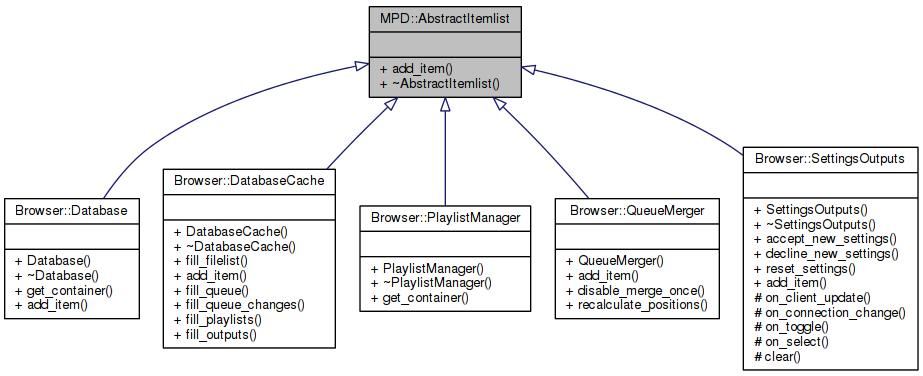
\includegraphics[width=\textwidth]{AbstractItemlist.png}
    \caption{Die AbstractItemList}
    \label{c_abstract_item_list}
\end{figure}

Für bestimmte Client Funktionen muss eine Nutzerklasse von \emph{AbstractItemlist} ableiten (siehe \ref{c_abstract_item_list}).
Leitet man ab, so muss die Methode add\_item(AbstractComposite * data) implementiert werden. 
Je nach Bedarf kann über \verb+static_cast<Zieltyp*>(data)+ der entsprechende Datentyp ,,rausgecasted'' werden.
Beim Aufruf von MPD::Client::fill\_queue ruft der Client die add\_item Methode für jeden 
Song den er vom Server bekommt auf. Die ableitende Klasse kann diese dann verarbeiten.

Dadurch werden alle Methoden von AbstractItemGenerator (bzw. die Klassen die davon ableiten) benutzbar.
%<Klassendiagramm, bzw. Klassen die es verwenden von Doxygen nehmen>

\subsubsection{AbstractItemGenerator}
%
%
%
% Hier wäre noch ein Sequenzdiagramm nötig,
% zB. für die Funktion fill_outputs( ) - beim Aufruf.

Lässt ableitende Klasse folgende Methoden implementieren:
Jede dieser Methoden ruft MPD::Playlist add\_item() von \emph{AbstractItemlist} auf um ihre Resultate weiterzugeben.
Sie erlaubt den Einsatz des \emph{Proxy-Patterns}.\footnote{http://en.wikipedia.org/wiki/Proxy\_pattern}
Andere Klassen können sich so als Client ,,ausgeben''.
Dies fand Anwendung bei der Klasse ,,DatabaseCache'' weiter unten.
\\
%<Sequenzdiagramm>   
Holt alle Songs der aktuellen Queue.
\begin{verbatim}            
    void fill_queue(AbstractItemlist& data_model);
\end{verbatim}

Holt alle geänderten Songs in der Queue seit der Version last\_version. Die Position des ersten geänderten Songs wird in first\_pos gespeichert. 
\begin{verbatim}
    void fill_queue_changes(AbstractItemlist& data_model,
                            unsigned last_version,
                            unsigned& first_pos);
\end{verbatim}

Holt alle gespeicherten Playlisten vom Server.
\begin{verbatim}              
    void fill_playlists(AbstractItemlist& data_model);
\end{verbatim}

Holt alle Audio Outputs vom Server.
\begin{verbatim}
    void fill_outputs(AbstractItemlist& data_model);
\end{verbatim}

Holt ein Listing aller Songs und Directories aus der Datenbank im Pfad 'path' (nicht rekursiv!)              
\begin{verbatim}
    void fill_filelist(AbstractItemlist& data_model, const char * path);
\end{verbatim}

%<Klassendiagramm, bzw. Klassen die es verwenden von Doxygen nehmen>

%-------------------------------------------
\newpage
\begin{figure}[htb!]
\subsubsection{AbstractComposite}
	\centering
        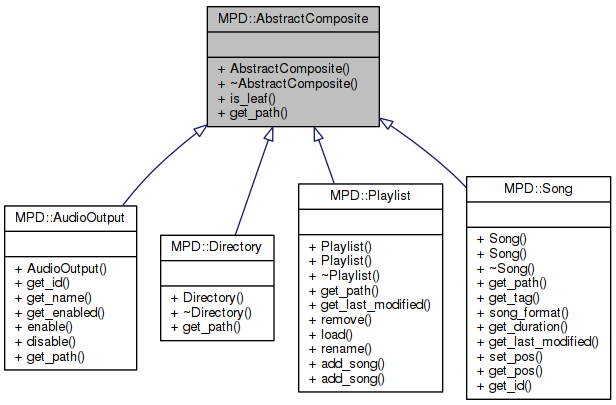
\includegraphics[width=\textwidth]{AbstractComposite.png}
	\caption{Klassendiagramm zu AbstractComposite}
	\label{c_abstract_composite}
\end{figure}

Vereinheitlicht Zugriff auf Komponenten verschiedenen Typs.
Die abstrakte Klasse (siehe Abb.: \ref{c_abstract_composite}) zwingt seine Kinder dazu eine \emph{get\_path()} Funktion zu implementieren die die Lage im virtuellen Filesystem des Servers angibt.
Der Hauptanwender dieser Klasse ist der Databasebrowser, bzw. der dahinter gelagerte Cache, da AbstractComposite es erlaubt Songs und Verzeichnisse gleich zu behandeln (vgl. Composite Pattern).
\\
Die erbende Klasse muss im Konstruktor angeben, ob es sich bei der Klasse um ein ,,File'' (\emph{true} für MPD::Song) oder um einen ,,Container'' (\emph{false} für MPD::Directory) handelt.
Diese ,,is\_leaf'' Eigenschaft kann später mit der Funktion \emph{is\_leaf()} abgefragt werden.

% <Klassendiagramm für alle Klassen die von AbstractComposite erben, siehe Doxygen>

%-------------------------------------------
\newpage
\begin{figure}[htb!]

\subsubsection{AbstractClientExtension}

	\centering
        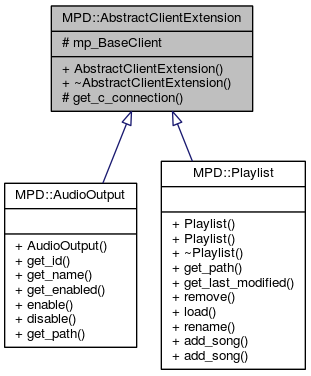
\includegraphics[scale=0.8]{AbstractClientExtension.png}
	\caption{Klassendiagramm zu AbstractClientExtension}
	\label{c_abstract_client_extension}
\end{figure}


Diese abstrakte Klasse erlaubt abgeleiteten Klassen ähnlich zum BaseClient eigene Kommandos zu implementieren (siehe \ref{c_abstract_client_extension}).
Dies geschieht indem die abstrakte Klasse eine Referenz auf den BaseClient im Konstruktor erwartet und speichert.
Ableitende Klassen können die \textit{protected} get\_c\_connection() Methode benutzen um eigene Kommandos zu implementieren.

\begin{verbatim}
   AbstractClientExtension(MPD::BaseClient& base_client)
\end{verbatim}

\emph{AbstractClientExtension} wird in diesem Entwurf von MPD::Playlist und MPD::AudioOutput benutzt.
Man kann allerdings darüber diskutieren dass dieses abstrakte Klasse der Modelschicht die Möglichkeit gibt zu ausgefeilte Logik zu implementieren, was nach dem MVC Paradigma nicht sein sollte.  
Da die Logik meist darin besteht einfache Kommandos an den Server zu schicken, wurde dieser Weg gewählt um 
den Entwurf zu vereinfachen.


%=============================================
